\chapter{Wcześniejsze rozwiązania}\label{r:losers}

%W chwili obecnej nie istnieje język dostosowany do potrzeb sumerologów.

Dotychczasowe rozwiązania problemu przeszukiwania bazy tabliczek opierają się o pomysł stworzenia formularza,
w którym, wypełniając odpowiednie pola, można określić jakich tabliczek szukamy.
Formularze różnią się od siebie przede wszystkim poziomem skomplikowania.
Im bardziej rozbudowany, tym więcej można w nim zdefiniować warunków dotyczących parametrów wyszukiwania,
ale jednocześnie tym trudniej z niego korzystać.
Z punktu widzenia dziedziny naszego problemu podstawową wadą takich rozwiązań jest 
brak możliwości tworzenia zapytań złożonych oraz brak elastyczności.
% TODO rozwinąć: co to jest brak elastyczności?


Poniżej przedstawimy dwie przykładowe strony internetowe oferujące wyszukiwanie za pomocą formularzy.


\section{The Cuneiform Digital Library Initiative \cite{cdli}}
\begin{figure}[h]
 \centering
 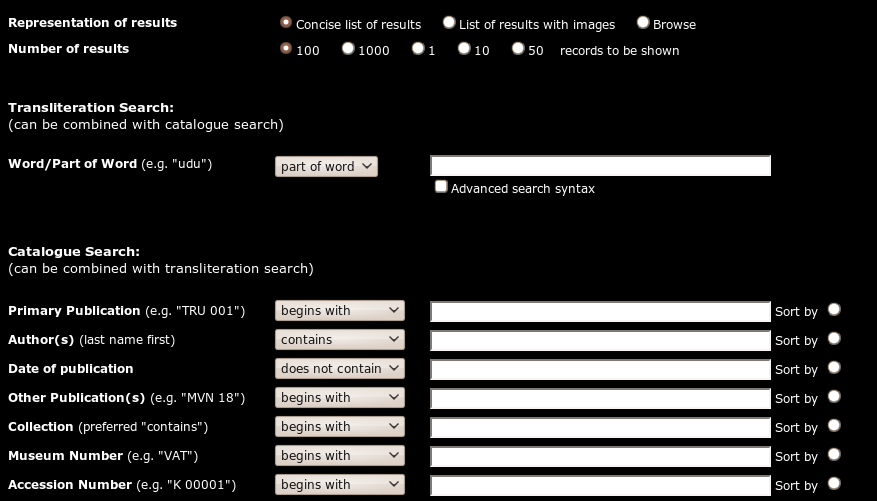
\includegraphics[width=300px]{../diagramy/cdli-search.png}
 % cdli-search.png: 877x501 pixel, 72dpi, 30.94x17.67 cm, bb=0 0 877 501
 \caption{Formularz wyszukiwania na stronie CDLI}
 \label{fig:cdli-search}
\end{figure}
Największą znaną nam bazą tekstów sumeryjskich jest The Cuneiform Digital Library Initiative (CDLI),
która zawiera ok. 225 tys. tabliczek.
Posiada stosunkowo rozbudowany formularz, 
który pozwala na wyszukiwanie po wielu parametrach tabliczki 
(m. in. po danych dotyczących czasu i miejsca powstania, komentarzach CDLI). 
Dla każdego parametru jest pole tekstowe z możliwymi opcjami wyszukiwania:
``begins with``, ``contains'', ''does not contain''.
Do wyszukiwania na podstawie treści tabliczki jest pole tekstowe z opcjami ``word``, ``part of word``.
Jest również checkbox ''advanced search syntax'', jednak brakuje wyjaśnienia jak go używać.
Nie można tworzyć bardziej skomplikowanych warunków dla poszczególnych parametrów
(np. nie można wyszukać tabliczek, które powstały w Uruk lub w Garshanie)
ani łączyć kilku zapytań w jedno zapytanie złożone.


\section{The Electronic Text Corpus of Sumerian Literature \cite{etcsl}}
\begin{figure}[h]
 \centering
 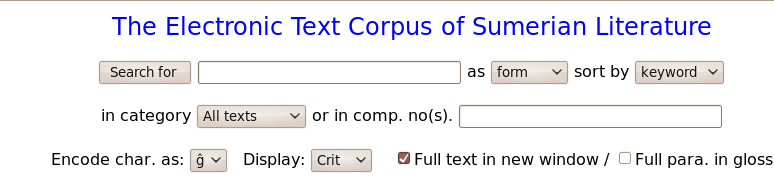
\includegraphics[width=300px]{../diagramy/etcsl-search.png}
 % etcsl-search.png: 774x182 pixel, 72dpi, 27.31x6.42 cm, bb=0 0 774 182
 \caption{Formularz wyszukiwania na stronie ETCSL}
 \label{fig:etcsl-search}
\end{figure}

The Electronic Text Corpus of Sumerian Literature (ETCSL) posiada znacznie mniejszą bazę niż CDLI,
składającą się z około 400 tekstów, głównie literackich.
Ma ograniczone możliwości wyszukiwania po metadanych - tylko po kategorii tekstu,
jednak udostępnia tworzenie bardziej skomplikowanych zapytań dotyczących treści tabliczki.
Pozwala określić typ wyszukiwanego słowa - do wyboru: form, lemma, label, pos, emesal, sign,
a także jego znaczenie w tekście (np. czy jest imieniem bóstwa) oraz część mowy, do której należy.
Można również wyszukiwać na podstawie fragmentu słowa.

